\documentclass[xetex,mathserif,serif]{beamer}
\usepackage{polyglossia}
\setdefaultlanguage[babelshorthands=true]{russian}
\usepackage{minted}
\usepackage{tabu}
\usepackage{forest}

\usepackage{textpos}
\setlength{\TPHorizModule}{1cm}
\setlength{\TPVertModule}{1cm}

\usetikzlibrary{arrows}

\useoutertheme{infolines}

\setmainfont{FreeSans}
\newfontfamily{\russianfonttt}{FreeSans}

\definecolor{links}{HTML}{2A1B81}
\hypersetup{colorlinks,linkcolor=,urlcolor=links}

\tabulinesep=1.2mm

\newcommand{\attribution}[1] {
	\begin{flushright}\begin{scriptsize}\textcolor{gray}{\textcopyright\, #1}\end{scriptsize}\end{flushright}
}

\title{Парадигмы программирования}
\author[Юрий Литвинов]{Юрий Литвинов \newline \textcolor{gray}{\small\texttt{yurii.litvinov@gmail.com}}}
\date{16.03.2018г}

\begin{document}
	
	\frame{\titlepage}

	\begin{frame}
		\frametitle{Математические модели вычислений}
		\begin{itemize}
			\item Что можно посчитать имея вычислительную машину неограниченной мощности?
			\item Формальные модели вычислений:
			\begin{itemize}
				\item Машина Тьюринга
				\item $\lambda$-исчисление Чёрча
				\item Нормальные алгорифмы Маркова
			\end{itemize}
		\end{itemize}
		Тезис Чёрча: <<Любая функция, которая может быть вычислена физическим устройством, может быть вычислена машиной Тьюринга>>
	\end{frame}

	\begin{frame}
		\frametitle{Машина Тьюринга}
		\begin{columns}
			\begin{column}{0.6\textwidth}
				\begin{itemize}
					\item Формально,
						$$M = (Q, \Gamma, b, \Sigma, \delta, q_0, F)$$
						$$\delta : (Q / F) × \Gamma \rightarrow Q × \Gamma × \{L, R\}$$
					\item Неформально:
					\begin{itemize}
						\item Бесконечная лента с символами из $\Sigma$ и $b$
						\item Считывающая головка
						\item Внутренняя память $Q$
						\item Таблица переходов $\delta$, которая по текущему состоянию из $Q$ и текущему символу на ленте из $\Gamma$ говорит машине, что делать:
						\begin{itemize}
							\item перейти в состояние
							\item записать символ на ленту
							\item сместиться влево/вправо
						\end{itemize}
					\end{itemize}
				\end{itemize}
			\end{column}
			\begin{column}{0.4\textwidth}
				\begin{center}
					\includegraphics[width=\textwidth]{turingMachine.png}
				\end{center}
			\end{column}
		\end{columns}
	\end{frame}

	\begin{frame}
		\frametitle{Архитектура фон Неймана}
		\begin{columns}
			\begin{column}{0.6\textwidth}
				\begin{itemize}
					\item Принцип последовательного программного управления
					\item Принцип однородности памяти
					\item Принцип адресуемости памяти
					\item Принцип двоичного кодирования
					\item Принцип жесткости архитектуры
				\end{itemize}
			\end{column}
			\begin{column}{0.4\textwidth}
				\begin{center}
					\includegraphics[width=\textwidth]{vonNeumannArchitecture.png}
				\end{center}
			\end{column}
		\end{columns}
	\end{frame}

	\begin{frame}
		\frametitle{Структурное программирование}
		\begin{itemize}
			\item Пришло на смену неструктурированному программированию в начале 70-х
			\begin{itemize}
				\item FORTRAN --- 1957 год, язык высокого уровня, но не структурный
			\end{itemize}
			\item Любая программа может быть представлена как комбинация
			\begin{itemize}
				\item последовательно исполняемых операторов
				\item ветвлений
				\item итераций
			\end{itemize}
			\item Статья Дейкстры <<Go To Statement Considered Harmful>> (1968г)
		\end{itemize}
	\end{frame}

	\begin{frame}
		\frametitle{Языки-представители}
		\begin{itemize}
			\item Алгол
			\item Паскаль
			\item Си
			\item Модула-2
			\item Ада
		\end{itemize}
	\end{frame}

	\begin{frame}[fragile]
		\frametitle{Подробнее: Ада}
		\begin{itemize}
			\item Разработан в начале 80-х по заказу минобороны США
			\item Особенности:
			\begin{itemize}
				\item Строгая типизация
				\item Минимум автоматических преобразований типов
				\item Встроенная поддержка параллелизма
			\end{itemize}
			\item Реализация: GNAT (\url{https://www.adacore.com/community})
		\end{itemize}
		\begin{minted}{ada}
    with Ada.Text_IO;
    use Ada.Text_IO;

    procedure Main is
    begin
        Put_Line ("Hello World");
    end Main;
		\end{minted}
	\end{frame}

	\begin{frame}[fragile]
		\frametitle{Ада, модульная система}
		\begin{minted}{ada}
package types is
    type Type_1 is private;
    type Type_2 is private;
    type Type_3 is private;
    procedure P(X: Type_1);
    ...
private
    procedure Q(Y: Type_1);
    type Type_1 is new Integer range 1 .. 1000;
    type Type_2 is array (Integer range 1 .. 1000) of Integer;
    type Type_3 is record
        A, B: Integer;
    end record;
end Types;
		\end{minted}
	\end{frame}

	\begin{frame}[fragile]
		\frametitle{Ада, многопоточность и рандеву}
		\begin{small}
			\begin{minted}{ada}
with Ada.Text_IO; use Ada.Text_IO;

procedure Main is
    task After is
        entry Go(Text: String);
    end After;

    task body After is
    begin
        accept Go(Text: String) do
            Put_Line("After: " & Text);
        end Go;
    end After;
begin
    Put_Line("Before");
    After.Go("Main");
end;
			\end{minted}
		\end{small}
	\end{frame}

	\begin{frame}[fragile]
		\frametitle{Ада, ограничения и контракты}
		\begin{minted}{ada}
type Not_Null is new Integer
    with Dynamic_Predicate => Not_Null /= 0;

type Even is new Integer
    with Dynamic_Predicate => Even mod 2 = 0;

function Divide (Left, Right : Float) return Float
    with Pre => Right /= 0.0,
         Post => Divide'Result * Right < Left + 0.0001
                 and then Divide'Result * Right > Left - 0.0001;
		\end{minted}
	\end{frame}

	\begin{frame}
		\frametitle{Объектно-ориентированное программирование}
		\begin{itemize}
			\item Первый ОО-язык --- Симула-67, были и более ранние разработки
			\item Популярной парадигма стала только в середине 90-х
			\item Развитие связано с широким распространением графических интерфейсов и компьютерных игр
		\end{itemize}
	\end{frame}

	\begin{frame}
		\frametitle{Основные концепции}
		\begin{itemize}
			\item Программа представляет собой набор объектов
			\item Объекты взаимодействуют путём посылки сообщений по строго определённым интерфейсам
			\item Объекты имеют своё состояние и поведение
			\item Каждый объект является экземпляром некоего класса
		\end{itemize}
	\end{frame}

	\begin{frame}
		\frametitle{Основные концепции (инкапсуляция)}
		\begin{itemize}
			\item Инкапсуляция --- сокрытие реализации от пользователя
			\item Пользователь может взаимодействовать с объектом только через интерфейс
			\item Позволяет менять реализацию объекта, не модифицируя код, который этот объект использует
		\end{itemize}
	\end{frame}

	\begin{frame}
		\frametitle{Основные концепции (наследование)}
		\begin{itemize}
			\item Наследование позволяет описать новый класс на основе существующего, наследуя его свойства и функциональность
			\item Наследование --- отношение <<является>> между классами, с классом-наследником можно обращаться так же, как с классом-предком
			\begin{itemize}
				\item Принцип подстановки Барбары Лисков
			\end{itemize}
		\end{itemize}
	\end{frame}

	\begin{frame}
		\frametitle{Основные концепции (полиморфизм)}
		\begin{itemize}
			\item Полиморфизм --- классы-потомки могут изменять реализацию методов класса-предка, сохраняя их сигнатуру
			\item Клиенты могут работать с объектами класса-родителя, но вызываться будут методы класса-потомка (позднее связывание)
		\end{itemize}
	\end{frame}

	\begin{frame}[fragile]
		\frametitle{Пример кода}
		\begin{minted}{cpp}
class Animal
{
    public:
        Animal(const string& name) { 
            this.name = name; 
        }

        void rename(const string &newName) { 
            name = newName; 
        }

        virtual string talk() = 0;

    private:
        string name;
};
		\end{minted}
	\end{frame}

	\begin{frame}[fragile]
		\frametitle{Пример кода (2)}
		\begin{minted}{cpp}
class Cat : public Animal
{
    public:
        Cat(const string& name) : Animal(name) {}
        string talk() override { return "Meow!"; }
};

class Dog : public Animal
{
    public:
        Dog(const string& name) : Animal(name) {}
        string talk() override { return "Arf! Arf!"; }
};
		\end{minted}
	\end{frame}

	\begin{frame}[fragile]
		\frametitle{Пример кода (3)}
		\begin{minted}{cpp}
...
Cat *cat1 = new Cat("Барсик");
Animal *cat2 = new Cat("Шаверма");
Dog *dog = new Dog("Бобик");

std::vector<Animal *> animals{cat1, cat2, dog};

for (Animal *animal : animals) {
    std::cout << animal->talk();
}
...
		\end{minted}
	\end{frame}

	\begin{frame}
		\frametitle{Языки-представители}
		\begin{itemize}
			\item Java
			\item C\#
			\item C++
			\item Object Pascal / Delphi Language
			\item Smalltalk
		\end{itemize}
	\end{frame}

	\begin{frame}
		\frametitle{Функциональное программирование}
		\begin{itemize}
			\item Вычисления рассматриваются как вычисления значения функций в математическом понимании (без побочных эффектов)
			\item Основано на $\lambda$-исчислении
		\end{itemize}
	\end{frame}

	\begin{frame}
		\frametitle{$\lambda$-исчисление}
		\begin{itemize}
			\item $\lambda$-исчисление --- формальный способ описать математические функции
			\begin{itemize}
				\item $\lambda{x}.2 * x + 1$ --- функция $x \rightarrow 2 * x + 1$
			\end{itemize}
			\item Функции могут принимать функции в качестве параметров и возвращать функции в качестве результата
			\item Функция от n переменных может быть представлена, как функция от одной переменной, возвращающая функцию от n - 1 переменной (карринг)
			\item Формальная система, не требующая математических оснований
			\begin{itemize}
				\item На самом деле, математика может быть построена на $\lambda$-исчислении
			\end{itemize}
		\end{itemize}
	\end{frame}

	\begin{frame}
		\frametitle{Языки-представители}
		\begin{itemize}
			\item Лисп (LIst PRocessing)
			\item ML (OCaml)
			\begin{itemize}
				\item F\#
			\end{itemize}
			\item Haskell
			\item Erlang
		\end{itemize}
	\end{frame}

	\begin{frame}
		\frametitle{Особенности}
		\begin{itemize}
			\item Программы не имеют состояния и не имеют побочных эффектов
			\begin{itemize}
				\item Нет переменных
				\item Нет оператора присваивания
			\end{itemize}
			\item Порядок вычислений не важен
			\item Циклы выражаются через рекурсию
			\item Ленивые вычисления
			\item Формальные преобразования программ по математическим законам
		\end{itemize}
	\end{frame}

	\begin{frame}[fragile]
		\frametitle{Пример на языке Haskell}
		Факториал:
		\begin{minted}{haskell}
fact :: Integer -> Integer 
fact 0 = 1 
fact n | n > 0 = n * fact (n - 1) 
		\end{minted}

		QSort:
		\begin{minted}{haskell}
sort [] = [] 
sort (pivot:rest) = sort [y | y <- rest, y < pivot] 
                    ++ [pivot]
                    ++ sort [y | y <- rest, y >=pivot] 

		\end{minted}
	\end{frame}

	\begin{frame}[fragile]
		\frametitle{F\#, мерджсорт}
		\begin{small}
			\begin{minted}{fsharp}
let rec merge l r =
    match (l, r) with
    | ([], r) -> r
    | (l, []) -> l
    | (x::xs, y::ys) -> if (x < y) then x::(merge xs r) else y::(merge l ys)
 
let rec mergesort l = 
    match l with
    | [] -> []
    | x::[] -> l
    | _ -> 
          let (left, right) = List.splitAt (List.length l / 2) l
          let ls = mergesort left
          let rs = mergesort right
          merge ls rs
			\end{minted}
		\end{small}
	\end{frame}

	\begin{frame}[fragile]
		\frametitle{F\#, бесконечная последовательность простых чисел}
		\begin{minted}{fsharp}
let isPrime number =
     seq {2 .. sqrt(double number)}
     |> Seq.exists (fun x -> number % x = 0) 
     |> not

let primeNumbers =
     Seq.initInfinite (fun i -> i + 2)
     |> Seq.filter isPrime
		\end{minted}
	\end{frame}

	\begin{frame}
		\frametitle{Логическое программирование}
		\begin{itemize}
			\item Программа представляет собой набор фактов и правил, система сама строит решение с использованием правил логики
			\begin{itemize}
				\item Использует логику предикатов как математическую формализацию
			\end{itemize}
			\item Создавалось в 60-х для решения задач искусственного интеллекта и экспертных систем
			\begin{itemize}
				\item Автоматическое доказательство теорем
			\end{itemize}
			\item Могут использоваться разные стратегии доказательства
			\begin{itemize}
				\item В общем случае, программа --- это набор фактов и правил + стратегия вывода, которая управляет тем, как новые факты получаются из существующих
				\begin{itemize}
					\item В формальной логике стратегия вывода обычно не важна, для компьютеров это критично
				\end{itemize}
			\end{itemize}
			\item Дедуктивные базы данных --- хранят факты и правила вывода
		\end{itemize}
	\end{frame}

	\begin{frame}
		\frametitle{Пролог}
		\begin{itemize}
			\item Появился в 1972 г. как научная разработка
			\item Реализации:
			\begin{itemize}
				\item SWI-Prolog (\url{http://www.swi-prolog.org/})
				\item Amzi Prolog (\url{http://www.amzi.com/})
				\item Turbo Prolog
			\end{itemize}
			\item Использует метод резолюций – последовательно перебирая правила и факты, пытается подобрать такой набор переменных, которые бы им удовлетворяли
			\begin{itemize}
				\item Пример:
				\begin{itemize}
					\item cat(tom)
					\item ?- cat(tom).

						Yes
					\item ?- cat(X).

						X = tom
				\end{itemize}
			\end{itemize}
		\end{itemize}
	\end{frame}

	\begin{frame}[fragile]
		\frametitle{Пример программы}
		\begin{minted}{prolog}
sibling(X, Y) :- parent_child(Z, X), parent_child(Z, Y).
parent_child(X, Y) :- father_child(X, Y).
parent_child(X, Y) :- mother_child(X, Y).
mother_child(trude, sally).
father_child(tom, sally).
father_child(tom, erica).
father_child(mike, tom).

?- sibling(sally, erica).
Yes
?- father_child(Father, Child).
		\end{minted}
	\end{frame}

	\begin{frame}[fragile]
		\frametitle{Императивное программирование}
		\begin{minted}{prolog}
?- write('Hello world!'), nl.
Hello world!
true.

program_optimized(Prog0, Prog) :-
    optimization_pass_1(Prog0, Prog1),
    optimization_pass_2(Prog1, Prog2),
    optimization_pass_3(Prog2, Prog).
		\end{minted}
	\end{frame}

	\begin{frame}[fragile]
		\frametitle{QSort}
		\begin{minted}{prolog}
quicksort(Xs, Ys) :- quicksort_1(Xs, Ys, []).

quicksort_1([], Ys, Ys).
quicksort_1([X|Xs], Ys, Zs) :-
    partition(Xs, X, Ms, Ns),
    quicksort_1(Ns, Ws, Zs),
    quicksort_1(Ms, Ys, [X|Ws]).
 
partition([K|L], X, M, [K|N]):-
    X < K, !,
    partition(L, X, M, N).
partition([K|L], X, [K|M], N):-
    partition(L, X, M, N).
partition([], _, [], []).
		\end{minted}
	\end{frame}

	\begin{frame}
		\frametitle{Рекурсивное программирование, РЕФАЛ}
		\begin{itemize}
			\item РЕкурсивных Функций АЛгоритмический
			\begin{itemize}
				\item В. Турчин, 1966г.
			\end{itemize}
			\item Ориентирован на символьные вычисления
			\begin{itemize}
				\item ИИ, перевод, манипуляции с формальными системами (лямбда-исчисление, например)
			\end{itemize}
			\item Использует нормальные алгорифмы Маркова в качестве математической формализации
			\item Программа записывается в виде набора функций
			\begin{itemize}
				\item Функция --- упорядоченный набор предложений
				\item Предложение состоит из шаблона и того, на что надо заменить шаблон
				\item Выражения в угловых скобках (активные выражения)
				\item Переменные
			\end{itemize}
			\item Вычисление продолжается, пока в <<поле зрения>> Рефал-машины не окажется выражение без угловых скобок
		\end{itemize}
	\end{frame}

	\begin{frame}[fragile]
		\frametitle{Рефал, пример}
		Hello, world:
		\begin{minted}{text}
$ENTRY Go { = <Hello>;}
Hello {
   = <Prout 'Hello world'>;
}
		\end{minted}
		\vspace{3mm}
		Палиндром:
		\begin{minted}{text}
Palindrom {
    s.1 e.2 s.1 = <Palindrom e.2> ;
    s.1 = True ;
    = True;
    e.1 = False ;
}
		\end{minted}
	\end{frame}

	\begin{frame}
		\frametitle{Стековое программирование}
		\begin{itemize}
			\item Язык Форт (Forth)
			\begin{itemize}
				\item Разработан в 60-х Чарльзом Муром <<для себя>>
				\item Был широко распространён для программирования встроенных систем и задач, естественным образом выражающихся в терминах стеков
				\begin{itemize}
					\item Синтаксический анализ
					\item Анализ естественных языков
				\end{itemize}
			\end{itemize}
		\end{itemize}
	\end{frame}

	\begin{frame}
		\frametitle{Форт, подробнее}
		\begin{itemize}
			\item Основной элемент программы: слово
			\item Форт-система состоит из словаря (набора слов) и стеков --- арифметического и командного (с их помощью производятся вычисления)
			\item Используется обратная польская нотация
		\end{itemize}
	\end{frame}

	\begin{frame}
		\frametitle{Примеры}
		\begin{columns}
			\begin{column}{0.82\textwidth}
				\begin{itemize}
					\item \mintinline{forth}|25 10 * 50 + .|

						Вывод: 300 ok
					\item \mintinline{forth}|: FLOOR5 ( n -- n' )   DUP 6 < IF DROP 5 ELSE 1 -| \\
						\mintinline{forth}|  THEN ;|
					\begin{itemize}
						\item то же самое на C:

						\mintinline{c}|int floor5(int v) { return v < 6 ? 5 : v - 1; }|
					\end{itemize}
					\item более красиво на Форте:

						\mintinline{forth}|: FLOOR5 ( n -- n' ) 1- 5 MAX ;|
					\item \mintinline{forth}|: HELLO  ( -- )  CR ." Hello, world!" ;|
				\end{itemize}
			\end{column}
			\begin{column}{0.18\textwidth}
				\begin{center}
					\includegraphics[width=\textwidth]{forthStack.png}
				\end{center}
			\end{column}
		\end{columns}
	\end{frame}

	\begin{frame}[fragile]
		\frametitle{Форт, пример}
		\begin{minted}{forth}
\ Напечатать знак числа
: .SIGN ( n -- )
   ?DUP 0= IF
     ." НОЛЬ"
   ELSE
     0> IF
     ." ПОЛОЖИТЕЛЬНОЕ ЧИСЛО" ELSE
     ." ОТРИЦАТЕЛЬНОЕ ЧИСЛО" THEN
   THEN
;
		\end{minted}
	\end{frame}

	\begin{frame}
		\frametitle{Реализации}
		\begin{columns}
			\begin{column}{0.8\textwidth}
				\begin{itemize}
					\item SwiftForth
					\begin{itemize}
						\item \url{https://www.forth.com/swiftforth/}
					\end{itemize}
					\item Gforth
					\begin{itemize}
						\item \url{http://www.gnu.org/software/gforth/}
					\end{itemize}
					\item Десятки других реализаций
					\begin{itemize}
						\item \url{http://www.forth.org/commercial.html}
					\end{itemize}
					\item Книжка
					\begin{itemize}
						\item Броуди Л. <<Начальный курс программирования на Форте>>
					\end{itemize}
				\end{itemize}
			\end{column}
			\begin{column}{0.2\textwidth}
				\begin{center}
					\includegraphics[width=\textwidth]{forthBookCover.png}
				\end{center}
			\end{column}
		\end{columns}
	\end{frame}

	\begin{frame}
		\frametitle{Визуальное программирование}
		\begin{itemize}
			\item Визуальные языки появились ещё до компьютеров
			\begin{itemize}
				\item Диаграммы потоков данных
				\item Сети Петри
			\end{itemize}
			\item Применяются прежде всего для моделирования, а не для программирования
			\begin{itemize}
				\item Описание архитектуры системы (UML, SysML, IDEFx)
				\item Описание бизнес-процессов (UML, BPMN)
				\item Описание схем баз данных (ER, ORM)
			\end{itemize}
			\item Есть и языки программирования: G (LabVIEW), Simulink, ДРАКОН, Scratch
			\item Предметно-ориентированные визуальные языки
			\begin{itemize}
				\item TRIK Studio
			\end{itemize}
		\end{itemize}
	\end{frame}

	\begin{frame}
		\frametitle{Пример (Matlab/Simulink)}
		\begin{center}
			\includegraphics[width=0.9\textwidth]{simulink.png}
		\end{center}
	\end{frame}

	\begin{frame}
		\frametitle{Пример (LabVIEW)}
		\begin{center}
			\includegraphics[width=0.8\textwidth]{labView.png}
		\end{center}
	\end{frame}

	\begin{frame}
		\frametitle{Пример (ДРАКОН)}
		\begin{center}
			\includegraphics[width=0.6\textwidth]{drakon.png}
		\end{center}
	\end{frame}

	\begin{frame}
		\frametitle{Визуальное моделирование}
		\begin{columns}
			\begin{column}{0.7\textwidth}
				\begin{itemize}
					\item Не ставит своей целью получить работающую программу
					\item Модель проще, чем нужно исполнителю
					\item Модель даже для сложной системы обозрима
					\item Система описывается с разных дополняющих друг друга точек зрения
					\begin{itemize}
						\item При этом описание системы остаётся целостным, визуальная модель --- это не просто картинка
					\end{itemize}
					\item Модели можно анализировать до реализации
					\item Могут быть сгенерированы заглушки классов и иногда даже реализации методов
				\end{itemize}
			\end{column}
			\begin{column}{0.3\textwidth}
				\begin{center}
					\includegraphics[width=\textwidth]{pointsOfView.png}
				\end{center}
			\end{column}
		\end{columns}
	\end{frame}

	\begin{frame}
		\frametitle{Пример высокоуровневой модели (UML)}
		\begin{center}
			\includegraphics[width=0.9\textwidth]{componentDiagram.png}
		\end{center}
	\end{frame}

	\begin{frame}
		\frametitle{Ещё пример (UML)}
		\begin{center}
			\includegraphics[width=\textwidth]{sequenceDiagram.png}
		\end{center}
	\end{frame}

	\begin{frame}
		\frametitle{UML, диаграммы классов}
		\begin{center}
			\includegraphics[width=0.6\textwidth]{classDiagram.png}
		\end{center}
	\end{frame}

	\begin{frame}
		\frametitle{Предметно-ориентированное моделирование}
		\begin{itemize}
			\item Специальные языки и инструменты для конкретной задачи или группы похожих задач
			\item Благодаря узости предметной области можно генерировать полностью работающую программу по диаграмме
			\begin{itemize}
				\item Зато оно работает только для этой предметной области
			\end{itemize}
			\item Могут программировать даже непрограммисты
		\end{itemize}
	\end{frame}

	\begin{frame}
		\frametitle{Пример: TRIK Studio}
		\begin{columns}
			\begin{column}{0.5\textwidth}
				\begin{itemize}
					\item Среда программирования роботов
					\item Программа --- набор элементарных команд
					\begin{itemize}
						\item Исполняются на реальном роботе по WiFi, Bluetooth, USB
						\item Генерируются в код на текстовом языке и загружаются на робот
						\item Исполняются на двумерной модели
					\end{itemize}
					\item Можно программировать только роботы
					\item Могут программировать даже дети, не умеющие ещё читать
				\end{itemize}
			\end{column}
			\begin{column}{0.5\textwidth}
				\begin{center}
					\includegraphics[width=\textwidth]{trikStudio.png}
				\end{center}
			\end{column}
		\end{columns}
	\end{frame}

\end{document}